\documentclass[a4paper]{article}
\usepackage{fullpage}
\oddsidemargin = -0.5in

\iffalse added for extra functionality \fi
\usepackage{booktabs}% http://ctan.org/pkg/booktabs
\newcommand{\tabitem}{~~\llap{\textbullet}~~}
\usepackage{graphicx,wrapfig,lipsum,mathtools}


\begin{document}
\section{What is HPC}
\subsection{Scientific Paradigms}
	\begin{itemize}
	\setlength{\itemsep}{-3pt}
	\item use in science, which cannot be done without
	\item classical science with paper and pen, todays science with HPC
	\item easier, cheaper, faster, safer to test things in simulations than in real life \\
	$\xrightarrow[]{}$ computational science\\
	\item no end to computational power needed (it can always be more accurate)
	\end{itemize}
	
\subsection{HPC examples}
	\begin{itemize}
	\setlength{\itemsep}{-3pt}
	\item weather \& fluid dynamics
	\item car-crash simulation
	\item business-analytics
	\item movie rendering
	\end{itemize}
	
	\paragraph{Big Data}
	is a new form of HPC. it is characterized by ither Huge amounts of data, fast generated
	data or a big variety of data. In this course Big Data will not be the main concern.\\
	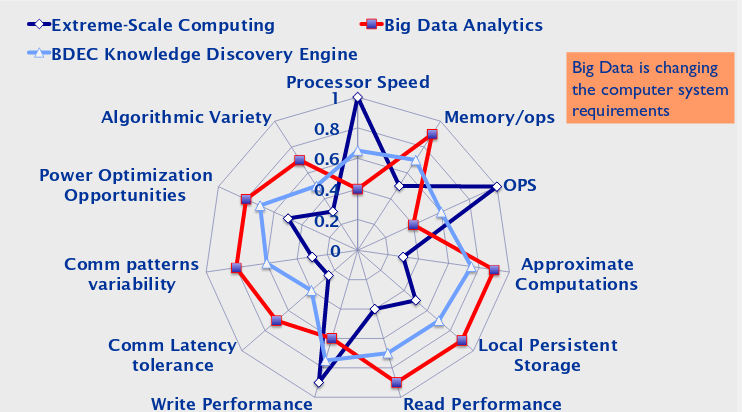
\includegraphics[width=400pt]{img/HPCRadar.png}\\\\

\section{Developments in Technology}
	\begin{tabular}{lll}
	CPU & getting better faster than & Memory\\
	& $\xrightarrow[]{}$ write algorithms to use data longer & \\
	& $\xrightarrow[]{}$ put more memory on CPU & \\
	Bandwidth & getting better faster than & Latency (speed of data retrieval after request)\\
	CPU & not getting better since & 2007\\
	& $\xrightarrow[]{}$ give CPU more cores&\\
	& $\xrightarrow[]{}$ new programing paradigmes&\\
	& $\xrightarrow[]{}$ GPUs \& FPAGs&\\
	\end{tabular}
\end{document}